\part{linux 基础知识}

在第一部门中先了解linux基础操作知识,他们包括系统知识,网络知识,


\chapter{系统基础}

\section{centos7 安装}

CentOS 7 网卡名不以eth0开始原因,是由于systemd 和 udev 引入了一种新的网络设备命名方式–一致网络设备命名(CONSISTENT NETWORK DEVICE NAMING) 。可以根据固件、拓扑、位置信息来设置固定名字,带来的好处是命名自动化,名字完全可预测,在硬件坏了以后更换也不会影响设备的命名,这样可以让硬件的更换无缝化。带来的不利是新的设备名称比传统的名称难以阅读。比如心得名称是enp5s0.

想要改为像centos6一样以eth0开始的名称有两种方法,在出现安装新系统的时候按下tab键,在kernel启动选项中增加 net.ifnames=0 biosdevname=0 


\begin{figure}[!ht]
    \centering    
     \caption{\label{Fig:async} Asynchronous I/O model}
    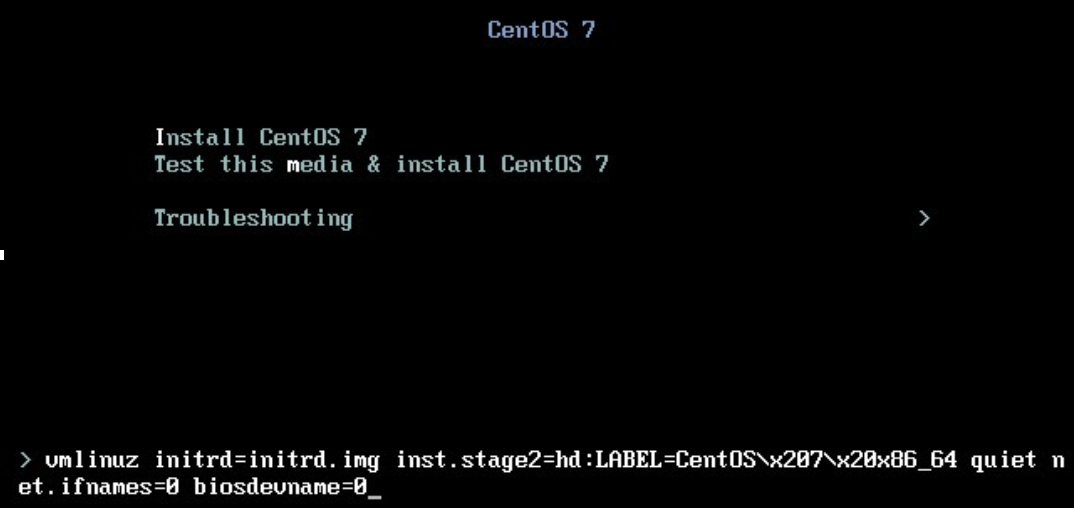
\includegraphics[width=0.8\textwidth]{./images/centos-bios.png}  
\end{figure}

当然,如果在安装时忘记操作了也可以在启动后操作。在 /etc/sysconfig/grub下相应位置加上这两个参数,然后再改网卡名既可

\begin{lstlisting}
GRUB_CMDLINE_LINUX=”rd.lvm.lv=vg0/swap vconsole.keymap=us crashkernel=auto  vconsole.font=latarcyrheb-sun16 net.ifnames=0 biosdevname=0 rd.lvm.lv=vg0/usr rhgb quiet”

grub2-mkconfig -o /boot/grub2/grub.cfg

\end{lstlisting}

安装完系统后一般需要关闭selinux, NetworkManager, firewalld, 需要安装net-tools, lsof, tcpdump, epel,

\subsection{桥接}

一、网卡桥接设置:

1、网卡配置文件:

[root@localhost /]# vim /etc/sysconfig/network-scripts/ifcfg-enp8s0

TYPE=Ethernet
DEVICE=enp8s0
NAME=enp8s0
BOOTPROTO=none
ONBOOT=yes
BRIDGE=br0

 2、网桥配置文件:

[root@localhost /]# vim /etc/sysconfig/network-scripts/ifcfg-br0

TYPE=Bridge
DEVICE=br0
BOOTPROTO=static
ONBOOT=yes
IPADDR=192.168.1.200
NETMASK=255.255.255.0
GATEWAY=192.168.1.1
DNS1=114.114.114.114


二、网卡绑定设置:

1、网卡配置文件01:

[root@localhost /]# vim /etc/sysconfig/network-scripts/ifcfg-enp6s0f0

TYPE=Ethernet
DEVICE=enp6s0f0
NAME=enp6s0f0
BOOTPROTO=none
ONBOOT=yes
USERCTL=no
MASTER=bond0
SLAVE=yes
2、网卡配置文件02:

[root@localhost /]# vim /etc/sysconfig/network-scripts/ifcfg-enp6s0f1

TYPE=Ethernet
DEVICE=enp6s0f1
NAME=enp6s0f1
BOOTPROTO=none
ONBOOT=yes
USERCTL=no
MASTER=bond0
SLAVE=yes
3、网桥配置文件:

[root@localhost /]# vim /etc/sysconfig/network-scripts/ifcfg-bond0

TYPE=Ethernet
DEVICE=bond0
BOOTPROTO=static
ONBOOT=yes
USERCTL=no
IPADDR=172.16.1.216
NETMASK=255.255.255.0
GATEWAY=172.16.1.1
DNS1=114.114.114.114

3. 在bond0基础上增加多个桥接网卡
[root@yw-qa-kvm-04 network-scripts]# cat ifcfg-bond0.300
BOOTPROTO=none
DEVICE=bond0.300
ONBOOT=yes
VLAN=yes
BRIDGE=virbr300
[root@yw-qa-kvm-04 network-scripts]# cat ifcfg-bond0.3960
BOOTPROTO=none
DEVICE=bond0.3960
ONBOOT=yes
VLAN=yes
BRIDGE=virbr3960

[root@yw-qa-kvm-04 network-scripts]# cat ifcfg-virbr300
TYPE=bridge
BOOTPROTO=static
DEVICE=virbr300
ONBOOT=yes
IPADDR=10.30.0.252
NETMASK=255.255.255.0
DELAY=0
[root@yw-qa-kvm-04 network-scripts]# cat ifcfg-virbr3960
TYPE=bridge
BOOTPROTO=static
DEVICE=virbr3960
ONBOOT=yes
IPADDR=10.18.61.252
NETMASK=255.255.255.0
DELAY=0


\section{磁盘分区与挂载}

\subsection{磁盘简介}
用于存储数据的物理设备便叫磁盘,磁盘接接口的不同可以分为:IDE,  SATA, SCSI, SAS.

\begin{itemize}
\item IDE的英文全称为“Integrated Drive Electronics”,即“电子集成驱动器”,
\item SCSI的英文全称为“Small Computer System Interface”
\item SATA(Serial ATA)又叫串口硬盘,PC机硬盘的主流趋势。
\item SAS(Serial Attached SCSI)即串行连接SCSI,是新一代的SCSI技术,此接口的设计是为了改善存储系统的效能、可用性和扩充性,并且提供与SATA硬盘的兼容性
\end{itemize}

磁盘内部由多个盘片,机械手臂,磁头,主轴马达组成。在读取数据时主轴马达驱动盘片转动,机械手臂可伸展来让磁头(head)读取数据,在盘片上存储数据,所以磁盘的容量便要看盘片的质量。

\begin{description}
	\item[磁道(Track)]:在每个盘片上由不同半经组成的同心圆叫做磁道,
	\item]扇区(Sector)]:每个磁道中被分隔成的最小的俱单位便是扇区每个扇区为512bytes
	\item[柱面(Cylinder)]:由多个盘片相同磁道所组成的圆柱面便是柱面
\end{description}

磁盘读取与写入数据时会按柱面来写入,只有柱面写完(读完)后才会切换磁道。
磁盘容量计算方式:Head * cylinder * Secor * 512bytes

每个磁盘的第一扇区非常重要,因为在该扇区存放着两个重要信息
1. 主引导分区(Master Boot Record, MBR) 有446bytes 主要用于安装引导加载程序
2. 分区表(Partition table) 记录整块磁盘分区状态,有64bytes

\subsection{磁盘分区}
由于分区表仅有64bytes所以只能记录4组记录区,每组记录区记录了该区段的启始与结束的柱面号码。所以每个磁盘只能分四个主(Primary)或扩展分区(Extended)。
而每个磁盘只允许有一个扩展分区,且扩展分区不能被格式化后存放数据,需要在扩展分区之上划分逻辑分区(Logical)。linux设备中的文件名1-4给主或者扩展分区预留,逻辑分区从5开始。

在linux下给磁盘分区的命令有`fdisk` 适合小于2T的磁盘分区, `parted` 擅长于大于2t 的磁盘分区。分区的实质便是修改分区表

\subsubsection{ fdisk 对磁盘分区}
使用命令`fdisk -cu /dev/sdb` 来进行对sdb分区,用命 -l来查看分区分区时的命令有

\begin{itemize}
\item  d   delete a partition 删除一个分区
\item  n   add a new partition       新增一个分区
\item  p   print the partition table 把分区打印出来
\item  q   quit without saving changes 不保存退出
\item  w   write table to disk and exit  保存分区并退出
\end{itemize}

这里需要注意在交互式分区过程中输错之后需要用**Ctrl + u**来撤消。 交互式实在太费事,这对于批量分区来说太费事可以用下面命令来一键搞定
\begin{lstlisting}
echo -e "n\np\n1\n\n+10G\nn\np\n2\n\n+20G\nw" |fdisk /dev/sdb
\end{lstlisting}

上一便仅是创建两个主分区,第一个分区给10G,第二个分区给20G,创建其它分区也类似

\subsubsection{ parted 对磁盘分区}
parted的操作都是实时的,也就是说你执行了一个分区的命令,他就实实在在地分区了,而不是像fdisk那样,需要执行w命令写入所做的修改, 所以进行parted的测试千万注意不能在生产环境中!
>传统的MBR(Master Boot Record)分区方式,有一个局限:无法支持超过2TB的硬盘的分区(或单个分区超过2TB)如果大于2T就要使用用GPT(Globally Unique Identifier Partition Table Format)分区的概念.

非交互式分区方式

\begin{lstlisting}
parted /dev/sdb  mklabel gpt yes
parted /dev/sdb  mkpart primary ext4 0 100  Ignore
parted /dev/sdb  mkpart primary linux-swap 101 8192 Ignore
parted /dev/sdb  mkpart logical ext4 8193 100GB  Ignore
parted /dev/sdb  mkpart logical ext4 101GB 3000GB Ignore
parted /dev/sdb  quit
\end{lstlisting}

\subsection{ 格式化与挂载}
磁盘分区好后,必须先格式化后才能挂载

\begin{lstlisting}
$ mkfs.ext4 /dev/sdb1
$ mkfs.ext4 /dev/sdb2

$ tune2fs -c -1 /dev/sdb1
tune2fs 1.41.12 (17-May-2010)
Setting maximal mount count to -1
#格式化后便可以挂载了
$ mount /dev/sdb1 /mnt
$ mount |grep --color=auto "/dev/sdb1"
/dev/sdb1 on /mnt type ext4 (rw)
\end{lstlisting}

在这里手动挂载后,系统重启后还需要再手动挂载一次,因为这里需要修改文件/etc/fstab 这个文件以达到开机自动挂载

磁盘被手动挂载之后都必须把挂载信息写入/etc/fstab这个文件中,否则下次开机启动时仍然需要重新挂载。 系统开机时会主动读取/etc/fstab这个文件中的内容,根据文件里面的配置挂载磁盘。这样我们只需要将磁盘的挂载信息写入这个文件中我们就不需要每次开机启动之后手动进行挂载了。挂载的限制
\begin{itemize}
\item  根目录是必须挂载的,而且一定要先于其他mount point被挂载。因为mount是所有目录的跟目录,其他木有都是由根目录 /衍生出来的。
\item  挂载点必须是已经存在的目录。
\item  挂载点的指定可以任意,但必须遵守必要的系统目录架构原则
\item  所有挂载点在同一时间只能被挂载一次
\item  所有分区在同一时间只能挂在一次
\item  若进行卸载,必须将工作目录退出挂载点(及其子目录)之外。
\end{itemize}

下面我们看看看/etc/fstab文件,这是我的linux环境中/etc/fstab文件中的内容

\begin{lstlisting}[language=bash]

$ cat /etc/fstab

#
# /etc/fstab
# Created by anaconda on Wed Oct 28 23:23:38 2015
#
# Accessible filesystems, by reference, are maintained under '/dev/disk'
# See man pages fstab(5), findfs(8), mount(8) and/or blkid(8) for more info
#
UUID=faba0886-9c24-430c-8ce5-f7980c283bbd /                       ext4    defaults        1 1
UUID=a2ea9c91-9424-4d8e-b15f-946ef8413877 /boot                   ext4    defaults        1 2
UUID=f11549e2-cd8a-4ec5-92ca-e8a83a16c87e swap                    swap    defaults        0 0
tmpfs                   /dev/shm                tmpfs   defaults        0 0
devpts                  /dev/pts                devpts  gid=5,mode=620  0 0
sysfs                   /sys                    sysfs   defaults        0 0
proc                    /proc                   proc    defaults        0 0
/dev/sdb1               /mnt                    ext4    defaults        0 0

\end{lstlisting}

可以看到fstab里一共有六列。

第一列 Device **Device**  是磁盘设备文件或者该设备的Label或者UUID
Label就是分区的标签,在最初安装系统是填写的挂载点就是标签的名字。可以通过查看一个分区的superblock中的信息找到UUID和Label name。
例如我们要查看/dev/sda1这个设备的uuid和label name
使用设备名称(/dev/sda)来挂载分区时是被固定死的,一旦磁盘的插槽顺序发生了变化,就会出现名称不对应的问题。因为这个名称是会改变的。不过使用label挂载就不用担心插槽顺序方面的问题。不过要随时注意你的Label name。至于UUID,每个分区被格式化以后都会有一个UUID作为唯一的标识号。使用uuid挂载的话就不用担心会发生错乱的问题了。

\begin{lstlisting}[language=bash]
$ dumpe2fs -h /dev/sda1
dumpe2fs 1.35 (28-Feb-2004)
Filesystem volume name:   /boot   #这个就是Label name
Last mounted on:
Filesystem UUID:          3b10fe13-def4-41b6-baae-9b4ef3b3616c    #UUID
Filesystem magic number:  0xEF53
Filesystem revision #:    1 (dynamic)
Filesystem features:      has_journal ext_attr resize_inode dir_index filetype needs_recovery sparse_super
Default mount options:    (none)
Filesystem state:         clean
#简单点的方式我们可以通过下面这个命令来查看
$ blkid /dev/sda1
/dev/sda1: LABEL="/boot" UUID="3b10fe13-def4-41b6-baae-9b4ef3b3616c" SEC_TYPE="ext3" TYPE="ext2"
\end{lstlisting}


第二列:Mount point 设备的挂载点,就是你要挂载到哪个目录下。

第三列: filesystem 磁盘文件系统的格式,包括ext2、ext3、ext3、reiserfs、nfs、vfat等. 生产场景中如果是大量小文件业务 首选 reiserfs。而 ext4 适合视频下载,流媒体,数据库,小文件业务

 ReiserFS是一个基于B状树的文件系统,拥有非常好的总体性能,特别是对于大量小文件。ReiserFS 拥有良好的伸缩性并具有日志功能。但该文件系统不再受到积极开发,不支持SELinux,基本上已被 Reiser4 取代。ReiserFS文件系统多年来一直用作一些发行版(包括SUSE)的默认文件系统,但现在用得少了。

 XFS文件系统拥有日志功能,包含一些健壮的特性,并针对可伸缩性进行了优化。XFS在RAM中强制缓存中转数据,因此如果使用 XFS,建议采用不间断电源供应。淘宝的数据库在使用此文件系统。

第四列:parameters 文件系统的参数

\begin{description}
	\item[Async/sync]设置是否为同步方式运行,默认为async
	\item[auto/noauto]当挂载mount -a 的命令时,此文件系统是否被主动挂载。默认为auto
	\item[rw/ro      ]是否以以只读或者读写模式挂载
	\item[exec/noexec]限制此文件系统内是否能够进行"执行"的操作
	\item[user/nouser]是否允许用户使用mount命令挂载
	\item[suid/nosuid]是否允许SUID的存在
	\item[Usrquota	]启动文件系统支持磁盘配额模式
	\item[Grpquota	]启动文件系统对群组磁盘配额模式的支持
	\item[Defaults	]同事具有rw,suid,dev,exec,auto,nouser,async等默认参数的设置
\end{description}

第五列:能否被dump备份命令作用, dump是一个用来作为备份的命令。通常这个参数的值为0或者1, 0代表不要做dump备份, 1代表要每天进行dump的操作, 2 代表不定日期的进行dump操作

第六列 是否检验扇区 开机的过程中,系统默认会以fsck检验我们系统是否为完整(clean). 0 不要检验,1 最早检验(一般根目录会选择),2 1级别检验完成之后进行检验


 以上会用到的命令会另一篇文章专门介绍下面仅罗列一些相关的命令
\begin{description}
	\item[格式]:mkfs, tune2fs, dumpe2fs
	\item[挂载]: mount umount /etc/fstab
	\item[磁盘检查], df, fsck,  e2fsck
	\item[调整文件大小] resize2fs
	\item[分区]: fdisk parted, partprobe, dd
\end{description}


 给swap增加容量

\begin{lstlisting}[language=bash]
dd if=/dev/zero  of=/tmp/swap bs=1M count=128
mkswap  /tmp/swap
swapon  /tmp/swap
\end{lstlisting}


机械磁盘读写磁盘数据的原理小结:
1. 磁盘是按照柱面为单位读写数据的, 既先读取同一个盘面的某一个磁道,读完之后如果数据没有读完,磁头也不会切换到其他
的磁道, 而是选择切换磁头,读取下一个盘面相同半径的磁道, 直到所有盘面的相同半径的磁道读取完成之后,如果数据还没有读写成,才会切换其他不同半径的磁道,这个切换磁道的过程称为寻道。
2. 不同磁头间的切换是电子切换, 而不同磁道间的切换需要磁头做径向动动,这个径向运动需要不进行电机调节,这个运行是机械的切换。

第一个硬盘   第二个硬盘  第三个硬盘 , 使用硬件RAID, LVM等工成一个或者多个虚拟磁盘,在系统中以块设备名体现/dev/sda

/dev/sdb  等, 在进行使用之前需要进行格式化(创建虚拟文件系统,不同系统使用的文件系统不一样,xfs,ext3,ext4),每一个分区都有各自的inode与block.以供系统使用。

英文单词, Head磁头, Sector扇区, Track 磁道,Cylinder柱面,Units单元块, Block数据块, Inode索引节点
buffer: 一般 用于写操作, 写缓冲

Raid0是条带化,把多个磁盘合起来组成一个大磁盘 支持1 块到多块盘,容量是所有磁盘之和,读写速度最快,没有冗余
Raid1 只支持偶数盘,镜像盘。 读写性能一般,成本高
Raid5 奇偶校验盘,最少三块,可以块一块盘,写入恨不能不高
Raid10,先做Raid1然后再做Raid0,保存备份以及数据量,最少4块盘,读写性能快,成本高。


\section{文件描述符及通配符}

\subsection{ 通配符}
  普通命令都可以用的特殊符号,不同的通配符有不同的意义,现在简单介绍在linux中不同的通配符的不同意义。

|符号  |意义   |符号  |意义    |符号  |意义|
|:----|:------|:----|:------|:----|:-----|
|*     |所有   |?     | 代表一个字符|; |命令分隔符|
|#     |注释   |竖线  |  管道 |~ | 用户家目录|
|-     |上一次目录|  $|  调用变量| /|  路径分隔符|
|>  >> |重定向,追加重定向|<  <<| 输入重定向,追加输入重定向|{}    |内容序列|
|'     |无变量转换功能    |"    |里面变量可以转换| `(反引号) | 把里面内容当做命令执行|

简单举例

	mkdir /etc/{bbc, blog}
	echo {a..z}

	a=1
	printf "$a\n"     #输出是1
	printf '$a\n'     #输出结果是 $a
	echo `date`       #输出结果是当时时间长格式


i_link 硬链接
i_count 进程


删除 文件需要看所在目录是否有写权限,没有写权限时是无法删除目录下面的文件

\section{文件权限}
chmod  只有文件的属主或root 才能来改变文件权限。

创建目录默认755
创建文件默认644

umask  修改默认权限通过八进制的数值来定义用户 创建文件或目录的默认权限

sed -n '65.69p' /etc/bashrc

666-umask
若umask部分位为基数,那么在结果的相应位置加一

777-umask

umask 对应数值表示的是禁止的权限,


特殊权限位(用户权限位)

以下内容不重要:

suid   s(x)    S 4
sgid   s(x)    S 2
sticky t(x)    T 1  沾滞位只能用ROOT来删除或创建。被创建的目录,任何用户可以在该目录下可以创建文件目录,但不能查看其它用户的内容,(/tmp)

授权方法 chmod (4000|2000|1000) /bin/rm  chmod (u|g|o)+(s|t )


seuid  权限位
当二进制命令执行
修改的是命令而非文件
仅对二进制命令才有作用。
suid权限仅在程序命令执行过程中有效。
suid是比较危险的功能,

sgid 是针对用户 组权限位的
对文件来说,sgid的功能如下

sgid 仅对二进制的命令程序有效
二进制命令或程序需要有可执行权限
执行命令在任意用户 可以获得该命令程序执行期间所属组的权限。

sgid 针对 目录
创建一个目录,要求在其 目录下创建的文件或目录的group继承该目录组
chmod 2755 /home/admins/


设置seuid
chmod 4755 /bin/rm

find / -perm 4755 -type f



更改文件属主与组 chown  chgrp


chown owrner:group   dirctory|file
chown :group       dirctory|file
chown owrner       dirctory|file

 groupadd test -g 501


\section{shell}
可执行文件开头第一行一般我们会指定用什么解释器来执行该文件比如shell角本的文件开头一般会加`#! /bin/sh`
如果是python文件(后缀名为.py)在第一行增加 `#! /usr/bin/python`

{toc}

### shell定义变量以及调用变量

运行shell 时会遇到三种变量
1. 局部变量, 在脚本或命令中定义,仅在当前shell实例中有效,其他shell启动的程序不能访问局部变量。
2. 环境变量,  所有的程序,包括shell启动的程序,都能访问环境变量,有些程序需要环境变量来保证其正常运行。必要的时候shell脚本也可以定义环境变量。
3. shell变量, 是由shell程序设置的特殊变量。shell变量中有一部分是环境变量,有一部分是局部变量,这些变量保证了shell的正常运行

定义变量时,变量名开始必须以[a-zA-Z]开始,中间不可以有空格或标点符号(可以用“\_”),变量名不可以使用bash的关键字。
调用变量,只需要在变量名前加"$"便可以了,考虑到解释器识别边界的问题,一般我们会在变量名外加大括号来确定变量名
删除变量可以用 `unset` 来取消变量的定义 .

现在我们便创建一个test.sh文件并且给它执行权限在里面输入以下内容

```
#! /bin/sh

#变量定义举例:
myName="sandow"
myUrl="http://magdre.github.io"
myAge=34
#调用变量
echo "hell everyone my name is $myName, my blog site is $myUrl,"
echo "Today, I'm ${myAge}years old"
#删除变量
unset myName
```


大括号(花括号)是为了让解释器识别变量名的边界,如果不加的话变量名就成了 $myAgeyears 这个变量名为空,输出来的便只有 **Todey, I'm old**  这样与期望值并不一样。

---

#### 在shell中的特殊变量名


|变量|  含义 |
|:--:|:----|
|\$0  | 当前脚本的文件名 |
|\$n  |传递给脚本或函数的参数。n 是一个数字,表示第几个参数,例 `$1` 。 如果超过10便需要写成 `${10}`|
|\$#  |传递给脚本或函数的参数个数。 |
|\$*  |传递给脚本或函数的所有参数。 |
|\$@  |传递给脚本或函数的所有参数。被双引号(" ")包含时,与 \$* 稍有不同,下面将会讲到。 |
|\$?  |上个命令的退出状态,或函数的返回值。 |
|\$$  | 当前Shell进程ID。对于 Shell 脚本,就是这些脚本所在的进程ID。 |

现在我们接着在test.sh里输下面内容

```
echo "File Name: $0"
echo "First Parameter : $1"
echo "Second Parameter : $2"
echo "Quoted Values: $@"
echo "Quoted Values: $*"
echo "Total Number of Parameters : $#"
```
我们在命令行输入
```
$ ./test.sh hello world
```
便可以得到下面结果
```
./tesh.sh
hello
world
hello world
hello world
2
```

#### 变量赋值与转换


|形式  |说明|
|:---|:----|
|\${var} | 变量本来的值 |
|\${var:-word} | 如果变量 var 为空或已被删除(unset),那么返回 word,但不改变 var 的值。 |
|\${var:=word} | 如果变量 var 为空或已被删除(unset),那么返回 word,并将 var 的值设置为 word。 |
|\${var:?message} | 如果变量 var 为空或已被删除(unset),那么将消息 message 送到标准错误输出,可以用来检测变量 var 是否可以被正常赋值。 若此替换出现在Shell脚本中,那么脚本将停止运行。 |
|\${var:+word} | 如果变量 var 被定义,那么返回 word,但不改变 var 的值。 |

#### shell里的运算
在原生bash中不支持简单的数学运算,但是可以通过其他命令来实现,例如 awk 和 expr,expr 最常用。
在使用expr时的格式为 `expr 1 + 2 `

a=10
b=20

**算术运算符**

|运算符 |说明 | 举例 |
|:--:|:--:|:---|
|\+   |加法 |`expr $a + $b` 结果为 30。|
|\-   |减法 |`expr $a - $b` 结果为 10。|
|\*   |乘法 |`expr $a \* $b` 结果为  200。|
|\/   |除法 |`expr $b / $a` 结果为 2。 |
|%   |取余 |`expr $b % $a` 结果为 0。 |
|=   |赋值 | a=\$b 将把变量 b 的值赋给 a。 |
|== |相等 |用于比较两个数字,相同则返回 true。 \[ $a == $b \] 返回 false。 |
|\!=  |不相等|用于比较两个数字,不相同则返回 true。 \[ $a != $b \] 返回 true。 |

**关系运算**

|运算符|说明|举例|
|:--:|:---|:---|
|-eq |检测两个数是否相等,相等返回 true | \[ \$a -eq \$b \] 返回 true |
|-ne |检测两个数是否相等,不相等返回 true | \[ \$a -ne \$b \] 返回 true |
|-gt |检测左边的数是否大于右边的,如果是,则返回 true | \[ \$a -gt \$b \] 返回 false|
|-lt |检测左边的数是否小于右边的,如果是,则返回 true | \[ \$a -lt \$b \] 返回 true |
|-ge |检测左边的数是否大等于右边的,如果是,则返回 true | \[ \$a -ge \$b \] 返回 false|
|-le |检测左边的数是否小于等于右边的,如果是,则返回 true | \[ \$a -le \$b \] 返回 true。 |

**逻辑运算**

|运算符|说明|举例|
|:--:|:--|:---|
|!  |非运算,表达式为 true 则返回 false | \[ \! false \] 返回 true |
|-o |或运算,有一个表达式为true则返回true | \[ \$a -lt 20 -o \$b -gt 100 \] 返回 true |
|-a |与运算,两个表达式都为true才返回true | \[ \$a -lt 20 -a \$b -gt 100 \] 返回 false |

**字符串运算符**

|运算符|说明|举例|
|:--:|:--|:---|
|=   |检测两个字符串是否相等,相等返回 true| \[ \$a = \$b \] 返回 false。 |
|!=  |检测两个字符串是否相等,不相等返回 true | \[ \$a != \$b \] 返回 true |
|-z  |检测字符串长度是否为0,为0返回 true |  \[ -z \$a \] 返回 false  |
|-n | 检测字符串长度是否为0,不为0返回 true |  \[ -n \$a \] 返回 true |
|str| 检测字符串是否为空,不为空返回 true | \[str \$a \] 返回 true  |

**文件测试运算符**

```
file="/var/www/tutorialspoint/unix/test.sh
```

|操作符|说明|举例|
|:--:|:--|:---|
|-b file | 检测文件是否是**块设备**文件,如果是,则返回 true | \[ -b \$file \] 返回 false |
|-c file |检测文件是否是**字符设备**文件,如果是,则返回 true| \[ -b \$file \] 返回 false |
|-d file |检测文件是否是**目录**,如果是,则返回 true| \[ -d \$file \] 返回 false |
|-f file |检测文件是否是**普通文件**(既不是目录,也不是设备文件),如果是,则返回 true| \[ -f \$file \] 返回 true。 |
|-g file |检测文件是否**设置了SGID位**,如果是,则返回 true| \[ -g \$file \] 返回 false|
|-k file |检测文件是否设置了**粘着位(Sticky Bit)**,如果是,则返回 true| \[ -k \$file \] 返回 false|
|-p file |检测文件是否是具名**管道**,如果是,则返回 true| \[ -p \$file \] 返回 false
|-u file |检测文件是否设置了**SUID位**,如果是,则返回 true| \[ -u \$file \] 返回 false。
|-r file |检测文件是否**可读**,如果是,则返回 true|\[ -r \$file \] 返回 true|
|-w file |检测文件是否**可写**,如果是,则返回 true| \[ -w \$file \] 返回 true|
|-x file |检测文件是否**可执行**,如果是,则返回 true| \[ -x \$file \] 返回 true|
|-s file |检测文件是否**为空**(文件大小是否大于0),不为空返回 true| \[ -s \$file \] 返回 true|
|-e file |检测文件(包括目录)**是否存在**,如果是,则返回 true| \[ -e \$file \] 返回 true|

#### shell 里处理字符

先定义一个变量:

```
string="sandow is a gentleman"
```

在python中用 `len(string)` 来计算字符串的长度,在shell里我们可以这样计算 `echo ${#string}`
在python中可以用 `string[1:4]` 来切片,在shell中 我们可以这样来实在 `${string:1:4}`
幸运的是这里index都是以0开头。所以切出来的值是相同的。
在python中用 `a.find("sandow")` 来查找字符,而在shell中可以这样写  `expr index "$string" sandow`

#### shell 中的数组

在shell中只可以建立一维数组,并且index从0开始,创建数组用小括号。

```
array_name=(value0 value1 value2 value3)
```

读取数组中某个值时可以用  `${array_name[index]}` 读取所有值可以用 “*” 或者 “@” 计算长度仅需要要array_name前加 “#” 与之前一样

#### shell 中的if 判断语法

```
if [ expression 1 ]
then
   Statement(s) to be executed if expression 1 is true
elif [ expression 2 ]
then
   Statement(s) to be executed if expression 2 is true
elif [ expression 3 ]
then
   Statement(s) to be executed if expression 3 is true
else
   Statement(s) to be executed if no expression is true
fi
```

#### case 语法
case 与excel里的case类似,取值先匹配每一个模式,模式匹配后,刚执行匹配模式相应命令,而不会继续其他模式。如果无一匹配模式,使用星号“\*”
来捕获该值,再执行后面的命令。 case的值后面必须为 `关键字 in`,每一模式必须以左括号结束,取值可以为变量或常数。匹配发现聚会符合某一模式后,其间所有命令开始执行直至遇到`;;`,结束。

```
case var in
pattern1)
    command1
    command2
    command3
    ;;
pattern2)
    command1
    command2
    command3
    ;;
*)
    command1
    command2
    command3
    ;;
esac
```

#### for 语法

```
for 变量 in 列表
do
    command1
    command2
    ...
    commandN
done
```
#### while 语法

```
while command
do
   Statement(s) to be executed if command is true
done
```
#### until 语法

```
until command
do
   Statement(s) to be executed until command is true
done
```

#### 函数语法
function 可有可无,不过做为一个合格的编程人员,有必要加上的。这才是规范。

```
function function_name () {
    list of commands
    [ return value ]
}
```

向函数内传递文件和上面一样 `function_name p1 p2 p3` 然后在函数内部用  `$n` 调用


\section{vim语法总结}
|语法| 描述|
|:---|:---|
|:wq!|强制保存|
|:q!|强制退出不保存|
|:set nu|显示行号|
| G |移动到最后一行|
|gg |移动到的第一行|
| 0 或者 ^ |移动到当前行的开头|
| $  |动到当前行的结尾|
| u  |取消上一次的动作|
| dd |删除一行|
|/patten |向下搜索|
|?  | 向上搜索|

下面是如何进入编辑模式
|语法| 描述|
|:---|:---|
| A  | 移动到行未并进入编辑模式|
| I  | 移到到行首并进入编辑模式|
| O  | 在当前行之前新建一行并进入编辑模式|
| o  | 在当前行之后新建一行并进入编辑模式

批量删除,以批量注释
命令模式下按 **ctal + v ** 移动光标选中需要修改的行,然后按**x** 或者 **d** 删除该内容或者按 **I** 进入编辑模式然后增加内容然后按esc退出后便可以看到所选区域都有显示

vim 下在编辑模式下也有自动补全功能便不是tab键,而是 `ctrl + n`
ctrl + o 跳到上一次修改的地方

\section{用户管理}


{:toc}

### useradd
命令描述: create a new user or update default new user information 新增一个用户或者更新创建用户的默认信息,
在不给定`-D`会新增一个用户,这时会更新系统里几个文件,见下面用户的家目录里面的文件会从/etc/skel下面copy过来。

|文件|说明|
|:---|:---|
|/etc/passwd |User account information.|
|/etc/shadow |Secure user account information.|
|/etc/group |Group account information.|
|/etc/gshadow | Secure group account information.|
|/etc/default/useradd | Default values for account creation.|
|/etc/skel/  | Directory containing default files.|
|/etc/login.defs |  Shadow password suite configuration.|

    [root@sandow ~]# useradd -D
    GROUP=100
    HOME=/home
    INACTIVE=-1
    EXPIRE=
    SHELL=/bin/bash
    SKEL=/etc/skel
    CREATE_MAIL_SPOOL=yes

    [root@sandow ~]# cat /etc/default/useradd
    # useradd defaults file
    GROUP=100
    HOME=/home
    INACTIVE=-1
    EXPIRE=
    SHELL=/bin/bash
    SKEL=/etc/skel
    CREATE_MAIL_SPOOL=yes

命令参数:

* -c, --comment COMMENT,对此用户备注,可以为任意字符
* -e, --expiredate EXPIRE_DATE 指定用户账号过期天数,时间格式为 YYYY-MM-DD
* -f, --inactive INACTIVE 密码过期后的缓存天数
* -M 不创建家目录
* -s, --shell SHELL,指定用户登录的shell,默认为空,让系统自动选择shell。
* -g, --gid GROUP 指定组,组名或者GID都可以
* -u, --uid UID 指定uid,必须惟一而且非负,默认是用最小的ID
* -U, --user-group Create a group with the same name as the user, and add the user to this group.

语法:

       useradd [options] LOGIN
       useradd -D
       useradd -D [options]

举例:

    [root@sandow ~]# useradd yusanpao -g newgroup  # 也可以用 -g 888
    [root@sandow ~]# id yusanpao
    uid=503(yusanpao) gid=888(newgroup) groups=888(newgroup)


### userdel
命令描述:delete a user account and related files,删除用户以及相关文件
命令参数:

* -f --force 强制删除用户,即使当前用户在登录状态,同时删除用户的家目录和邮件
* -r --remove 删除用户家目录和邮件

命令语法

       userdel [options] LOGIN

举例:

### passwd
命令描述: passwd - update user’s authentication tokens,修改用户的密码
命令参数:

* --stdin
* -d 删除用户密码,仅对root有效
* -n 密码的最小生效时间
* -x 密码的最大生效时间
* -w 提醒用户密码过期
* -i 密码过期后使用的天数


### groupadd - create a new group

命令描述: 增加一个新组
命令参数:

* -g, --gid GID 指定组ID,这个数字必须是惟一的,如果有`-O`,那么这个参数可以不惟一

命令语法:

    groupadd [options] group

涉及的文件有:

* /etc/group  Group account information.
* /etc/gshadow Secure group account information.
* /etc/login.defs Shadow password suite configuration.

举例:

    [root@sandow ~]# groupadd -g 888 newgroup
    [root@sandow ~]# tail -1 /etc/group
    newgroup:x:888:
    [root@sandow ~]# tail -1 /etc/gshadow
    newgroup:!::

说明:
/etc/group 是一个文本文件,它定义了系统中组的信息,它的每行所包含的意思有 `group_name:passwd:GID:user_list`
user_list用“,”号分开

### groupdel

命令描述: delete a group , groupdel会个性group,gsandow两个文件,如果组中有用户,必须先删除用户再删除组
命令语法: groupdel group
举例:

```
    [root@sandow ~]# groupdel newgroup
    groupdel: cannot remove the primary group of user 'yusanpao'
    [root@sandow ~]# userdel -r yusanpao
    [root@sandow ~]# groupdel newgroup
    [root@sandow ~]# tail -1 /etc/group
    OP:x:502:
```



### 用户查询相关命令

**users** print the user names of users currently logged in to the current host

    $ users
    root root root yuyingcai yuyingcai
    id  users w who last lastlog groups

**who** show who is logged on

    $ who -H
    NAME     LINE         TIME             COMMENT
    yuyingcai pts/0        2015-11-10 01:24 (10.0.0.1)
    root     pts/2        2015-10-30 02:24 (10.0.0.1)
    root     pts/3        2015-10-30 02:52 (10.0.0.1)
    yuyingcai pts/4        2015-11-10 00:00 (10.0.0.1)
    root     pts/5        2015-11-10 00:35 (10.0.0.1)

**w** Show who is logged on and what they are doing.

```
 01:32:28 up  6:16,  6 users,  load average: 0.00, 0.00, 0.00
USER     TTY      FROM              LOGIN@   IDLE   JCPU   PCPU WHAT
yuyingca pts/0    10.0.0.1         01:24   26.00s  0.06s  0.00s man w
root     pts/1    10.0.0.1         01:32    0.00s  0.06s  0.00s w
root     pts/2    10.0.0.1         30Oct15  1:19m  0.29s  0.05s -bash
root     pts/3    10.0.0.1         30Oct15 10days  0.07s  0.00s man useradd
yuyingca pts/4    10.0.0.1         00:00    1:32m  0.04s  0.04s -bash
root     pts/5    10.0.0.1         00:35   56:25   0.11s  0.00s man userdel
```


**last**  show listing of last logged in users

参数

* -f file Tells last to use a specific file instead  of /var/log/wtmp.
* -t YYYYMMDDHHMMSS 显示出指定日期下的用户登录信息

```
$ last -5
root     pts/1        10.0.0.1         Tue Nov 10 01:32   still logged in
yuyingca pts/0        10.0.0.1         Tue Nov 10 01:24   still logged in
yuyingca pts/0        10.0.0.1         Tue Nov 10 01:24 - 01:24  (00:00)
yuyingca pts/0        10.0.0.1         Tue Nov 10 01:24 - 01:24  (00:00)
yuyingca pts/8        10.0.0.1         Tue Nov 10 00:53 - 01:24  (00:30)
```


**lastlog** reports the most recent login of all users or of a given user

```
$ lastlog -u root
Username         Port     From             Latest
root             pts/1    10.0.0.1         Tue Nov 10 01:32:26 +0800 2015
```

lastlog formats and prints the contents of the last login log /var/log/lastlog
Last  searches  back  through  the file /var/log/wtmp


### su
命令描述:run a shell with substitute user and group IDs 切换用户

* -, -l, --login make the shell a login shell, clears all envvars except for TERM, initializes HOME, SHELL,  USER,  LOGNAME and PATH

### 为普通用户授权
因root权力太大,所以一般会为普通用户授权,从而减少不必要的安全问题,我们可以用visudo来修改用户权限。
使用visudo,相当于修改/etc/sudoers这个文件,但是visudo可以检查语法,所以一般都会用visudo来配置用户权限
![权限](sudo.jpg)

    [root@sandow ~]# ll /etc/sudoers
    -r--r-----. 1 root root 4057 Oct 29 18:47 /etc/sudoers

visudo 里一些内容说明


|行数 |用途        |语法|
|:----|:----|:----|
|16G |用户(组,前加“%”)别名    | User_Alias ADMINS = jsmith, mikem, %yunying |
|13G |主机别名     | Host_Alias FILESERVERS = fs1, fs2  |
|    |           | Host_Alias MAILERVERS = fs1, fs2  |
|16G |运行角色别名 | Runas_Alias  OP = root  |
|23G |命令别名    | Cmnd_Alias SOFTWARE = /bin/rpm, /usr/bin/up2date, /usr/bin/yum |
|98G |设置用户权限 | ADMINS       fs1=(OP)  SOFTWARE |
|    |           | ADMINS       fs1=(OP)  NOPASSWD: SOFTWARE |
|    |           | yunying      fs1=(OP)  /usr/sbin/*, !/usr/sbin/halt |
|56G |  ssh -t   |  Defaults    requiretty|

多个命令可以用","隔开 用"!" 用来禁止使用某个命令,必须放到最后。

    [root@sandow db]# visudo -c
    /etc/sudoers: parsed OK

    [sandow@sandow ~]$ sudo -l
    User sandow may run the following commands on this host:
        (ALL) /user/sbin/useradd, (ALL) /ser/sbin/userdel

sudo
-l 检查被授予的权限

-K 清空时间戳,之后用sudo还需要输密码。


简历里要加上如下项目经验:
二、服务器用户权限管理改造方案与实施项目
1.在了解公司业务流程后,提出权限整改解决方案改进公司超级权限root泛滥的现状。
2.我首先撰写了方案后,给老大看,取得老大的支持后,召集大家开会讨论。
3.讨论确定可行后,由我负责推进实施。
4.实施后效果,公司的服务器权限管理更加清晰了(总结维护)。
5.制定了账号权限申请流程及权限申请表格。

项目实战:简历中的经验说明
三、服务器日志审计项目提出与实施
1.权限权限方案实施后,权限得到了细化控制,接下来进一步实施对所有用户日志记录方案。
2.通过sudo和syslog(rsyslog)配合实现对所有用户进行日志审计并将记录集中管理(发送到中心日志服务器)。
3.实施后让所有运维和开发的所有执行的sudo管理命令都有记录可查,杜绝了内部人员的操作安全隐患。


---

### 日志审计

任何用户,执行的任何操作记录,(录像,回放)
1。 sudo 配合 rsyslog 服务 , 进行日志审计,
2。 在bash解释器程序里嵌入一个监视器,让所有审计的用户记录其执行的命令相关信息。



日志相关:rsyslog,Awstats,flume logstash scribe kafka,storm,ELK(Elasticsearch+Logstash+Kibana)
http://oldboy.blog.51cto.com/2561410/775056
收集日志软件ELK

rsyslog


跳板机、堡垒机:

开源跳板机(堡垒机)Jumpserver部署详解
http://blog.51cto.com/zt/658
CrazyEye
http://3060674.blog.51cto.com/3050674/1700814


日志相关:rsyslog,Awstats,flume logstash scribe kafka,storm,ELK(Elasticsearch+Logstash+Kibana)

实际配置
Defaults        logfile=/var/log/sudo.log

\section{磁盘}
Jupyter Notebook
磁盘结构图
Last Checkpoint: 2015年10月30日
(autosaved)
Current Kernel Logo
Python 3
File
Edit
View
Insert
Cell
Kernel
Widgets
Help


### 磁盘管理
​
磁盘的外部
sync;sync;reboot
​
​
buffer写入缓冲区
cache读取缓存区
![io](IO.png)
​
服务 器 dell , hp, ibm.
企业级SAS硬盘,
​
​
不提供访问的可以用SATA盘。
​
千万不要用SATA磁盘来做在线高并发服务的数据存储或数据业务,
把磁盘从sata(raid5) 换成SAS(raid10)
​
磁盘的容量=
 一个磁道的容量=扇区数*512bytes
 一个盘面的容量=磁道数*扇区数*512bytes
 磁盘的容量=盘面数*一个盘面的容量
​
 磁盘的容量=磁头数*磁道数*扇区数*512bytes
          255 heads * 1044 cylinders * 63 sectors/track
​
​
[root@sandow ~]# fdisk -l
​
Disk /dev/sda: 8589 MB, 8589934592 bytes
255 heads, 63 sectors/track, 1044 cylinders
Units = cylinders of 16065 * 512 = 8225280 bytes
Sector size (logical/physical): 512 bytes / 512 bytes
I/O size (minimum/optimal): 512 bytes / 512 bytes
Disk identifier: 0x0001e36d
​
   Device Boot      Start         End      Blocks   Id  System
/dev/sda1   *           1          26      204800   83  Linux
Partition 1 does not end on cylinder boundary.
/dev/sda2              26         914     7134208   83  Linux
Partition 2 does not end on cylinder boundary.
/dev/sda3             914        1045     1048576   82  Linux swap / Solaris
​
### 磁盘读写原理
​
寻道很慢,一个磁道到另一个磁道
​
​
磁头读数据按照柱面进行的。
​
### raid0
​
raid 技术
redundant array of inexpensive disk  (disk array)
​
容量更大,性能更高,有冗余
​
![](raid.png)
​
​
​
LVM逻辑卷管理,最大用途是可以管理磁盘的容量,让磁盘分区可以随意放大或者缩小。
​
RAID0  又称为Stripe条带化,它在所有raid级别中有最高的存储性能。
至少有1块物理磁盘,一般用来做RAID的不同磁盘大小。最好 一样。
生产中使用单盘,要做成RAID0。否则可能无法使用
​
​
### raid1
mirror 或mirroring镜像。至少两块盘。做好raid1,的容量为最小那块硬盘的容量。存储时同时写入两块磁盘,实现了数据完整备份,但相对降低了写入性能。 听说可以并发。
​
### raid 5
RAID 5是一种存储性能、数据安全和存储成本兼顾的存储解决方案。
最少三块盘。采用基偶校验
RAID 5是一种存储性能、数据安全和存储成本兼顾的存储解决方案。
RAID 5是把数据和相对应的奇偶校验信息存储到组成RAID5的各个磁盘上,并且奇偶校验信息和相对应的数据分别存储于不同的磁盘上。当RAID5的一个磁盘数据发生损坏后,利用剩下的数据和相应的奇偶校验信息去恢复被损坏的数据。
​
### raid10

​

\section{buffer cache区别}
cache:  一般 用于读操作, 读缓存。提高数据读取速度

CPU: L1 L2 L3  : CPU cache 位于内存与CPU之间。 CPU把内存中的数据读取到cache上,然后下次从cache读取,这样比读内存更快。
buffer 缓冲区,用于提高速度不同传输速度。 cpu把数据写到内存的磁盘缓存区 然后系统启动一个进程(pd flash)把内存的数据写到硬盘。
其目的都是解决速度不一致的问题。 有的太快,有的太慢。他们之前进行IO操作时,需要用buffer cache来提高IO操作,首先cache来读缓存,buffer写缓冲,写到离目的地最近的地方,然后再写到目的地。


浏览器第一次必须获取到资源后,然后根据返回的信息来告诉如何缓存资源,可能采用的是强缓存,也可能告诉客户端浏览器是协商缓存,这都需要根据响应的header内容来决定的。

第一次请求

\begin{figure}[!ht]
    \centering    
     \caption{\label{Fig:async} Asynchronous I/O model}
    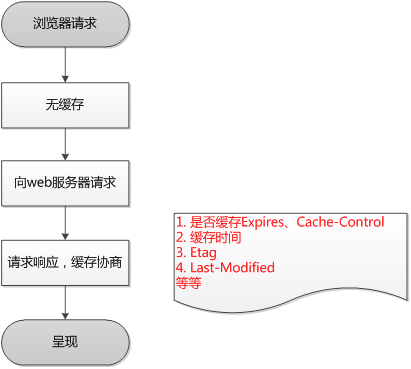
\includegraphics[width=0.8\textwidth]{./images/firstRequest.png}  
\end{figure}

下一次请求

\begin{figure}[!ht]
    \centering    
     \caption{\label{Fig:async} Asynchronous I/O model}
    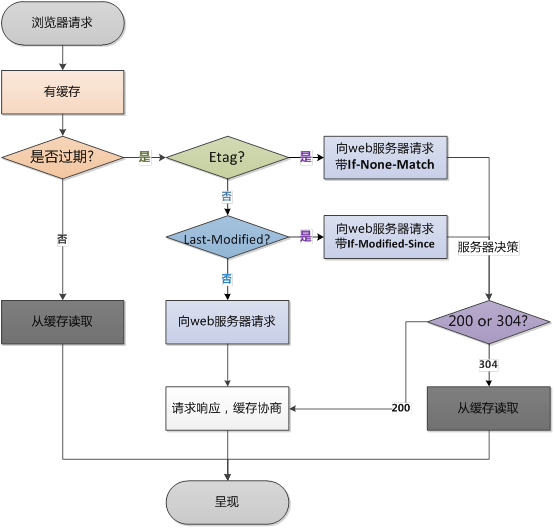
\includegraphics[width=0.8\textwidth]{./images/nextRequest.png}  
\end{figure}

\subsection{强缓存}

运维了解到此基础就OK, 需要了解更深可以查看网上资源

https://www.zhihu.com/question/20790576

https://www.cnblogs.com/wonyun/p/5524617.html

\section{linux系统命令}

用户权限分配

用户/组   主机    可以切换的用户角色	命令
root     ALL=     (ALL)			ALL
User_Alias  Host_Alias    Runas_Aliase  Cmad_Alias  
mikem
%groupname

